\section{Method}
In this section, we firstly show that the we can make sure that there is no overlapped points on target surface by enforcing the mapping to be injective. 
Then we propose the cycle regularization technique and explain in details (as shown in Figure~\ref{fig:net}) about how we respectively apply this general technique onto AtlasNet \cite{atlasnet} and Pixel2Mesh \cite{pixel2mesh}, whose network structures are quite different from each other.

\subsection{Injective mapping and self-overlapped points}
\label{subsec:inj}
Start with the definition of injective mapping at \textbf{Definition}~\ref{def:injective}, we can intuitively induce the conclusion that given a predefined surface with $ X =\{\mathbf{x}~|~\mathbf{x}$ is a point on the predefined surface $ \} $, a target surface with $ Y =\{\mathbf{y}~|~\mathbf{y}$ is a point on the target surface $ \} $ and a function $f:X \rightarrow Y$. If $\exists$ $ \mathbf{a},\mathbf{b} \in X$, $\mathbf{a} \neq \mathbf{b}$ and $f(\mathbf{a}) = f(\mathbf{b})$ (i.e. the overlapped points on target surface exists) then by definition, $f$ is not an injective function. Equivalently (as the converse negative proposition), we can make sure there is no self-overlapped points on the target surface by enforcing $f$ to be injective.
\begin{m_def}
\label{def:injective}
Let $f$ be a function whose domain is a set $X$. The function $f$ is said to be injective provided that
\begin{equation}
\forall a,b \in X, f(a) = f(b) \Rightarrow a = b.
\end{equation}
Equivalently, 
\begin{equation}
\forall a,b \in X, a \neq b \Rightarrow f(a) \neq f(b).
\end{equation}
\end{m_def}

\subsection{Cycle regularization}
\label{subsec:cyclereg}
\begin{m_thm}
\label{thm:injective}
functions with left inverses are always injective. That is, given $f:X \rightarrow Y$, if there is a function $g:Y \rightarrow X$ such that,
\begin{equation}
\label{equ:injective}
\forall x \in X,~g(f(x)) = x,
\end{equation}
then $f$ is injective.
\end{m_thm}

Based on \textbf{Theorem}~\ref{thm:injective}, we turn an injective constraint to our cycle regularization term as:
\begin{equation}
\label{equ:cycle_term}
cycle_X(f,g)=\sum_{\mathbf{x}\in X}||g(f(\mathbf{x})) - \mathbf{x}||_2^2.
\end{equation}
In mesh reconstruction networks, our term can be illustrated as in Figure~\ref{fig:issue}(b), 

By minimizing this term to zero:
\begin{equation}
f^*,g^* = \arg\min_{(f,g)} cycle_X(f,g)
\end{equation}
we can get the $f^*$ that has the left inverse function $g^*$, therefore $f^*$ is injective. 

\begin{figure*}[htbp]
	\centering
	\includegraphics[width=\linewidth]{img/opt/opt}
	\caption{Visualize convergence of optimization: When optimized with our cycle regularization term, the term take effect after only few iterations. It not only keep the mapping injective in optimization but also correct the self-intersection from the initialization. When optimized without cycle regularization term, the surface usually converge to a surface with self-intersection.}
	\label{fig:opt}
\end{figure*}

However, it is never possible to actually minimize a regularization term to zero, especially in training neural networks. But when this term is minimized to sufficiently small then we can construct $g^*$ that is the left inverse function of $f^*$ and guarantee that $f^*$ is injective. An example of such case is that when the regularization term is so small that $g(f(\mathbf{x}))$ is closer to $\mathbf{x}$ than any other point in $X$. Such example can be summarized by \textbf{Proposition}~\ref{prop:nearest}.

\begin{m_prop}
	\label{prop:nearest}
	Given sets $X$ and $Y$ that are subset of Euclidean space $\mathcal{R}^3$, function $f:X \rightarrow Y$  and function $g:Y \rightarrow X$, if
	\begin{equation}
	\exists~g, || g(f(\mathbf{x})) - \mathbf{x} ||_2^2 \leq \min_{\mathbf{b} \in X}|| g(f(\mathbf{x})) - \mathbf{b} ||_2^2,
	\end{equation}
	then $f$ is injective.
\end{m_prop}

\textbf{Proposition}~\ref{prop:nearest} can be proved by simplely composite nearest neighbor with the function $g$. We can construct nearest neighbor function $l: \mathcal{R}^3 \rightarrow X $ as:
\begin{equation}
\forall \mathbf{a} \in \mathcal{R}^3, l(\mathbf{a}) = \arg\min_{\mathbf{b} \in X} || \mathbf{a} - \mathbf{b} ||_2^2
\end{equation}
then
\begin{equation}
\begin{aligned}
&|| g(f(\mathbf{x})) - \mathbf{x} ||_2^2 \leq \min_{\mathbf{b} \in X}|| g(f(\mathbf{x})) - \mathbf{b} ||_2^2\\
&\Rightarrow \mathbf{x} = \arg\min_{\mathbf{b} \in X}|| g(f(\mathbf{x})) - \mathbf{b} ||_2^2\\
&\Rightarrow l(g(f(\mathbf{x}))) = \mathbf{x}\\
\end{aligned}
\end{equation}
then $g^*(\mathbf{y}) = l(g(\mathbf{y}))$ is the left inverse of $f$, therefore $f$ is injective.

\noindent\textbf{Remaining gap}
Even when the condition in Proposition~\ref{prop:nearest} is met after optimization, there is still no guarantee for $f$ being injective over the continue surface. The reason is that when we turn Equ.~(\ref{equ:injective}) into Equ.~(\ref{equ:cycle_term}), we actually create a theoretical gap. 
The the constraint in Equ.~(\ref{equ:injective}) is defined over continue surface, while the term in  Equ.~(\ref{equ:cycle_term}) is defined on discrete point set. In order to fill in the gap, we randomly sample $X$ from the predefined surface in training phase instead of minimizing the cycle regularization for any specific set of $X$. Sampling different $X$ from predefined surface is somehow already employed by AtlasNet (Ever since VAE\cite{VAE}, random vector as input is commonly used to encode latent variation in generation networks.). For Pixel2Mesh, we add such sampling in the inverse decoding, we could have added it in original network in a similar way as AtlasNet. We choose not to do so to advocate that our cycle regularization is a general regularization technique and it can work along with surface mesh generation networks without altering the original network. Our controlled experiment validates that such random sampling is crucial for our cycle regularization technique.

\subsection{Implementation along with networks}

As stated in AtlasNet \cite{atlasnet}, it is possible to use multilayer perceptron with ReLU nonlinearities and enough hidden units to approximate any shape within a small positive error $\epsilon$. In practice, we employ another 3D surface decoder to approximate $g$. Then we explain how we implement this technique for AtlasNet and Pixel2Mesh respectively. Generally speaking, we reuse the network structures from their network respectively and show that our cycle regularization is a general technique for this type of networks.

\noindent\textbf{AtlasNet} Depending on a shape representing feature $\mathbf{s}$, the AtlasNet use point-wise MLP
$f$ with parameters $\theta_f$ to learn to map points in $X=\{\mathbf{x}| \mathbf{x}$ are points uniformally sampled from predefined surface $P\}$ to points in $Y=\{\mathbf{y}| \mathbf{y}$ are points uniformally sampled from surface $S\}$. In implementation, $P$ is the surface of a 3D sphere. $S$ is the target surface, which is usually the surface of an object in AtlasNet \cite{atlasnet} and in this paper. Then we use another point-wise MLP $g$ with parameters $\theta_g$ to map points from $Y$ back to $X$. Along with our cycle regularization  total loss function for AtlasNet can be written as:

\begin{equation}
\begin{aligned}
\label{equ:atlascycle}
\mathcal{L}_{(X,Y)}(\theta_f,\theta_g) &= \sum_{\mathbf{x} \in X} \min_{\mathbf{y} \in Y}|| f_{\theta_f}(\mathbf{x};\mathbf{s}) - \mathbf{y} ||_2^2 \\ &+ \sum_{ \mathbf{y} \in Y}\min_{ \mathbf{x} \in X} || f_{\theta_f}(\mathbf{x};\mathbf{s}) - \mathbf{y} ||_2^2 \\ &+ \lambda\sum_{\mathbf{x} \in X}||g_{\theta_g}(f_{\theta_f}(\mathbf{x};\mathbf{s});\mathbf{s}) - \mathbf{x}||_2^2,
\end{aligned}
 \end{equation}
In which, the shape representation feature is simply concatenated to each point so that the $f$ and $g$ is depending on a global shape representing feature $\mathbf{s}$. $\lambda$ is the weight for cycle regularization. In AtlasNet, $\mathbf{s}$ is generated from either PointNet \cite{resnet} for auto-encoding or ResNet-18 \cite{resnet} for single view reconstruction. In implementation $g$ is a MLP with same number of units in hidden layers as $f$, as shown in Figure~\ref{fig:net}.

\noindent\textbf{Pixel2Mesh}
Comparing to AtlasNet, Pixel2Mesh \cite{pixel2mesh} use a more complicate network structure. In order to implement cycle regularization along with Pixel2Mesh, we need to cope with such design of network and use cycle regularization term in each level of point density.
As shown in Figure~\ref{fig:net}), Pixel2Mesh uses three blocks of graph based convolution residual network ($f_1,f_2,f_3$) to map mesh based features to target surface at three different level of point density. To be compatible with such framework, we also use three point-wise MLP as inverse decoder and form our regularization term as:
\begin{equation}
\begin{aligned}
\mathcal{L}_{cycle}(\theta_f,\theta_g) 
&= \sum_{\hat{\mathbf{x}} \in \hat{X}_1}||g_{1}(\hat{\mathbf{y_1}},\mathbf{s}_1) - \hat{\mathbf{x}}||_2^2\\
&+ \sum_{\hat{\mathbf{x}} \in \hat{X}_2}||g_{2}(\hat{\mathbf{y_2}},\mathbf{s}_2) - \hat{\mathbf{x}}||_2^2\\
&+ \sum_{\hat{\mathbf{x}} \in \hat{X}_3}||g_{3}(\hat{\mathbf{y_3}},\mathbf{s}_3) - \hat{\mathbf{x}}||_2^2,\\
\end{aligned}
\end{equation}
in which $\hat{\mathbf{x}}$ and $\hat{\mathbf{y}_l}$ are sampled as convex combination of vertexes in each triangle as: 
\begin{equation}
\begin{aligned}
&\hat{\mathbf{x}} = \sum^{N=3} w_n\mathbf{x}_n, \\
&\hat{\mathbf{y}_l} = \sum^{N=3} w_nf_l(\mathbf{x}_n,\mathbf{s}_l),\\
&\sum^{N=3} w_n = 1
\end{aligned}
\end{equation}
\begin{figure*}[htbp]
	\centering
	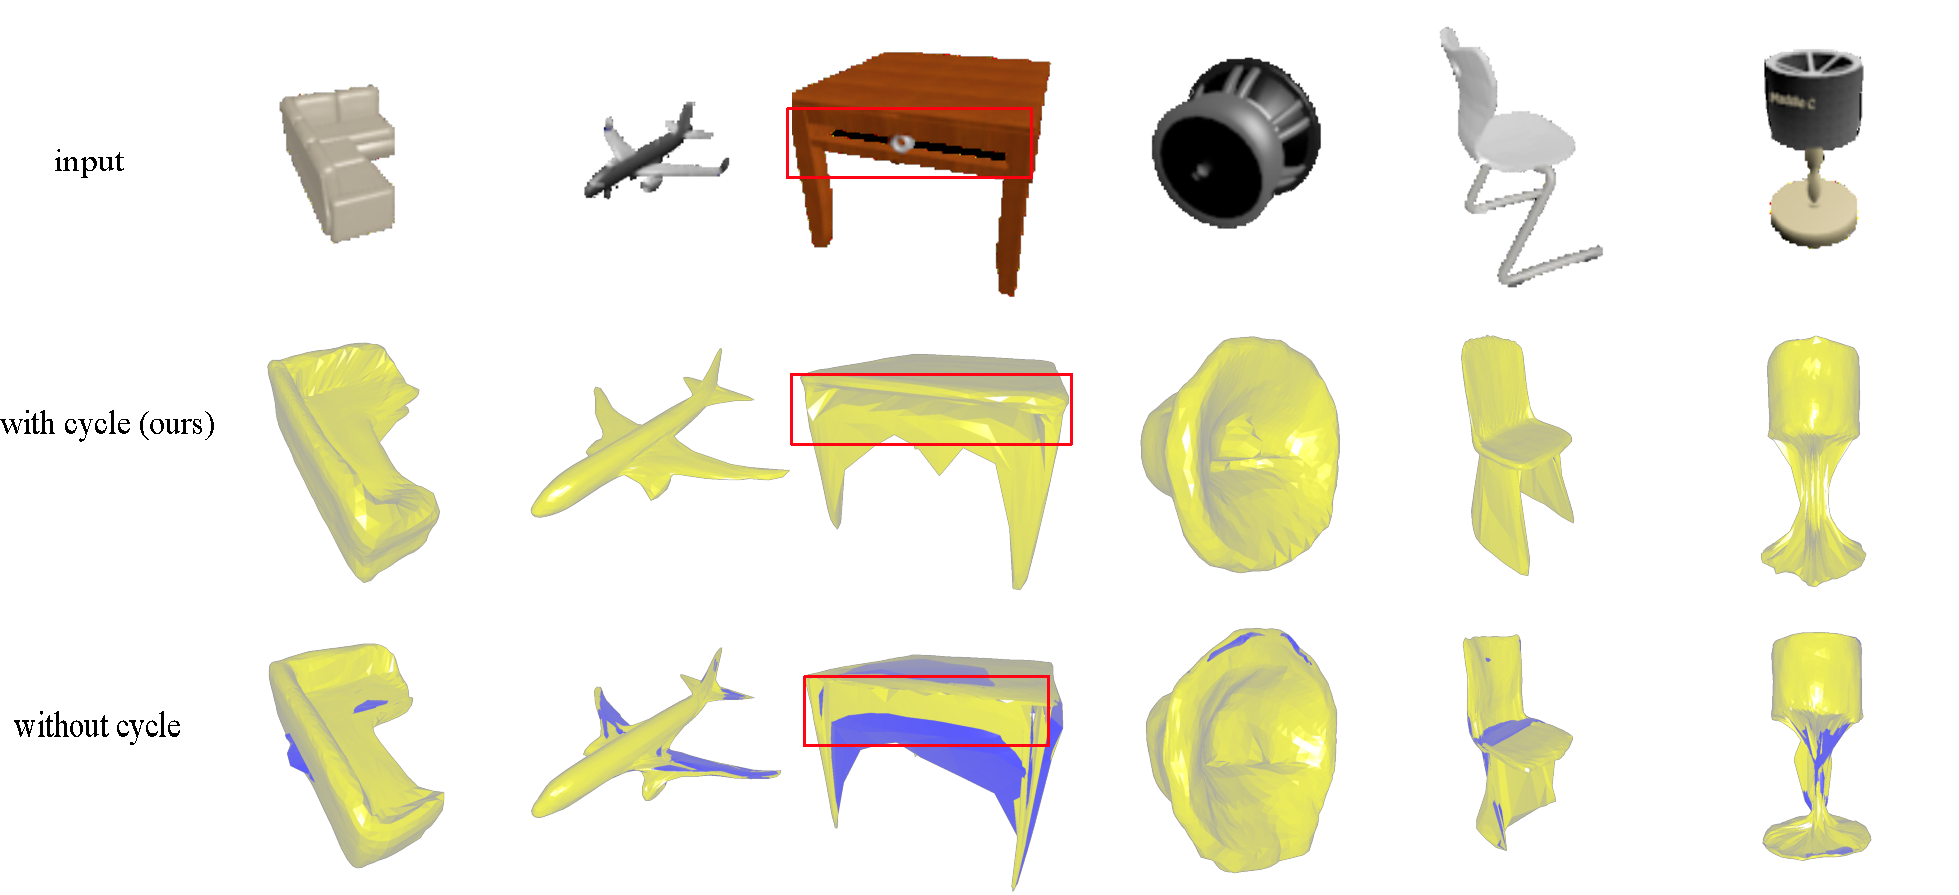
\includegraphics[width=\linewidth]{img/atlas/svr}
	\caption{Cycle regularization on AtlasNet: All the visualized cases here are selected from the test set of AtlasNet. Some meshes' view direction are manually adjusted to better expose the differences. The red rectangles are highlighting a case (the table) in which more details are preserved than the original network because we are enforcing the surface to be free of self-intersection with our cycle regularization term}
	\label{fig:svr}
\end{figure*}
the combination coefficients $w_n$ are randomly generated by kept consistent for $\hat{\mathbf{x}}$ and $\hat{\mathbf{y}_l}$ in each level $l$. $\theta_f$ is the whole parameters for $f_1,f_2,f_3$. $\theta_g$ is the whole parameters for $g_1,g_2,g_3$. $\mathbf{s}_1,\mathbf{s}_2,\mathbf{s}_3$ are features extracted from different layers of VGG-16 based on input point positions $X_1,X_2,X_3$ in original network. $\hat{X}_1,\hat{X}_2,\hat{X}_3$ are the sets of sampled points at each level. 
As we have mentioned in Sec~\ref{subsec:cyclereg} \emph{Remaining gap}, random sampling from predefined surface is crucial for our technique. Since Pixel2Mesh do not include such sampling in their method, we have to add it in our inverse decoding. In our inverse decoding we do not directly map the vertexes from target surface back to predefined surface as we did for AtlasNet. Instead, we map the sampled points $\hat{\mathbf{y}_l}$ from each face back to the corresponding samples $\hat{\mathbf{x}}$. The correspondence between $\hat{\mathbf{x}}$ and $\hat{\mathbf{y}_l}$ are ensured to be locally injective by using same set of convex combination coefficients $w_n$ for the sampling. We multiply our regularization term with weight $\lambda$ and add it to original loss function of Pixel2Mesh. For more details, please go to our supplemental material for the code of this implementation.
